\documentclass{beamer}
\usepackage{HECbeamer}
% \usepackage{pgfpages}
% \pgfpagesuselayout{4 on 1}[letterpaper, landscape, border shrink=5mm]
\title[\color{white}{MATH 60604A \S~7d - Cox proportional hazard model}]{\texorpdfstring{MATH 60604A \\Statistical modelling \\ \S~7d - Cox proportional hazard model}{MATH 60604A \\ Statistical modelling \\ \S~7d - Cox proportional hazard model}}
\author{}
\institute{HEC Montréal\\
Department of Decision Sciences}
\date{} 

\begin{document}
\frame{\titlepage}
% \begin{frame}
%  
% \end{frame}

\begin{frame}
\frametitle{Motivation}
\begin{itemize}
% \item The most commonly employed estimator of the survival function with non-informative right-censoring is Kaplan--Meier estimator.
\item What could we do if we wanted to measure the effect of explanatory variables $\mathrm{X}_1, \ldots, \mathrm{X}_p$ on the survival?
\begin{itemize} 
\item with categorical variables (and a lot of observations), we could estimate the survival function in each sub-group using Kaplan--Meier's estimator.
\item this approach does not work if $\mathrm{X}_j$ is continuous or the number of observations per group is small.
\end{itemize}
\end{itemize}
\end{frame}
% 
% \begin{frame}
% \frametitle{Cox proportional hazard model}
% \begin{itemize}
% \item Le modèle de Cox à risques proportionnels est un modèle \alert{semi-paramétrique} pour la fonction de risque $h(t)$. 
% \begin{itemize}
% \vp \vp
% \item C'est un modèle semi-paramétrique car il comprend à la fois une partie paramétrique et une partie non-paramétrique.
% \item La partie paramétrique du modèle est paramétrisée en terme de coefficients de régression $\beta_1, \ldots, \beta_p$, qui mesure les effets des variables explicatives sur la survie. 
% \end{itemize}
% \end{itemize}
% \end{frame}

\begin{frame}
\frametitle{Cumulative hazard function}

For $T$ continuous${}^*$, we define the cumulative hazard function as
\begin{align*}
H(t) = \int_{0}^{t} h(u) \d u = \int_0^t \frac{f(u)}{S(u)}\d u = -\ln\{S(t)\}
\end{align*}
and we can write the survival function  
\begin{align*}
S(t) = \exp\{-H(t)\}.
\end{align*}


We can write the log likelihood in terms of the (cumulative) hazard function
\begin{align*}
\ell(\bs{\theta}) = \sum_{i=1}^n \{\delta_i \ln h(t_i; \bs{\theta}) - H(t_i; \bs{\theta})\}
\end{align*}
\end{frame}


% \begin{frame}
% \frametitle{Fonction de risque}
% \begin{itemize}
% \item Pour un temps de survie $T$, la \alert{fonction de survie} est $S(t) = \P{T>t}$
% \item[] et la \alert{fonction de répartition} est $F(t) = \P{T\leq t}$
% 
% \item Rappel: on peut écrire la fonction de survie en terme de la fonction de répartition:
% \begin{align*}
% S(t) = 1 - F(t)
% \end{align*}
% \item La \alert{fonction de risque} (ou \alert{taux de défaillance} ou \alert{taux de risque}) est définie comme 
% \begin{align*}
% h(t) = \lim_{\delta \to 0} \frac{\P{t < T<t + \delta \mid T>t}}{\delta} = \lim_{\delta \to 0} \frac{1}{\delta}\frac{\P{t<T<t + \delta}}{\P{T>t}}
% \end{align*}
% \item On peut interpréter la fonction de risque comme étant la probabilité instantanée de ``mourir'' au temps $t$, compte tenu de la survie jusqu'au temps $t$.
% %\item \emph{We can think of the hazard rate as being the instantaneous probability of ``dying'' at temps $t$, given survival to temps $t$. }
% \end{itemize}
% \end{frame}

% \begin{frame}
% \frametitle{Fonction de risque}
% \begin{itemize}
% \item Quand $T$ est continue, on peut montrer que la fonction de risque est en fait
% \begin{align*}
% h(t) = \frac{-\d \ln S(t) }{\d t}
% \end{align*}
% \item On peut donc écrire la \alert{fonction de survie} en terme de la \alert{fonction de risque}:
% \begin{align*}
% S(t) = \exp\left\{ - \int_0^t h(u) \d u \right\}
% \end{align*}
% \item Alors, si on connait la fonction de survie, on peut établir la fonction de risque, et vice versa. 
% \item Connexion entre la courbe de survie et la fonction de risque:
% \begin{itemize}
% \vp \vp
% \item un taux de risque plus faible à $t$ implique une probabilité plus faible que l'événement (ex. la mort) survienne; la courbe de survie a une pente moins prononcée à $t$
% \item un taux de risque plus élevé implique une plus grande probabilité que l'événement (ex. la mort) survienne; la pente de la courbe de survie est plus abrupte à $t$.
% \end{itemize}
% \end{itemize}
% \end{frame}

\begin{frame}
\frametitle{Proportional hazard assumptions}
In the proportional hazard model, the hazard is parametrized as
\begin{align*}
 h(t; \mathbf{x}_i) = h_0(t)\exp(\mathbf{x}_i\bs{\beta})
\end{align*}
where
\bi \item the baseline hazard $h_0(t)$ is the only term that varies through time.
\item the \alert{proportional hazard} assumption implies that the ratio $h(t; \mathbf{x}_i)/h(t; \mathbf{x}_j)$ is constant regardless of time $t$.
\item the interpretation of the effect of explanatory variables is simpler because these effects don't vary over time.
\item this assumption is restrictive and must be validated in practice, but it is particularly convenient.
\ei

\textbf{Note:} there is no intercept in the Cox proportional hazard model: the latter is included in $h_0(t)$.
% Avec l'hypothèse de risque proportionnels, la fonction de survie devient
% \[
% S(t; \mathbf{x}_i) = \exp\left\{H_0(t_j)\right\}^{\exp(\mathbf{x}_i\bs{\beta})}
% \] 
% et la fonction de densité 
% \begin{align*}
% f(t; \mathbf{x}_i) = \exp(\bs{\beta}\mathbf{x}_i) h_0(t) S_0(t)^{\exp(\bs{\beta}\mathbf{x}_i)}. 
% \end{align*}
\end{frame}
\begin{frame}
 \frametitle{Derivation of the proportional hazards}
 
We consider observed failure times $0 \leq t_1 < \cdots < t_D$, assuming no ties to simplify the derivation.


The baseline cumulative hazard
\[
H_0(t) = \sum_{j: t_j \leq t} h_0(t_j),
\] is a step fonction with jumps only at the observed failure times.

We consider
\bi 
\item $\mathcal{R}_j$, the set of individuals at risk $t_j$
\item $\delta_i$, a binary indicator worth $1$ for the observed failure and $0$ if the observation is right-censored.
\ei

\end{frame}
\begin{frame}
 \frametitle{Likelihood of the Cox proportional hazard model}
 Let $h_j = h_0(t_j)$. The log likelihood is 
 \begin{align*}
  \ell(\bs{h}, \bs{\beta}) &= \sum_{i=1}^n \left\{ \delta_i \ln \{\exp(\mathbf{x}_i \bs{\beta})h_i\}-\exp(\mathbf{x}_i \bs{\beta})H_0(t_j)\right\} 
  \\& =  \sum_{i=1}^n \left\{ \delta_i \mathbf{x}_i \bs{\beta} + \delta_i \ln h_i -h_i \sum_{j \in \mathcal{R}_i}\exp(\mathbf{x}_j \bs{\beta})\right\} 
 \end{align*}
\bi
\item Since we are primarily interested in the effect of explanatories $\mathbf{X}$, we treat $h_1,\ldots, h_D$ as nuisance parameters.
\item 
If $\bs{\beta}$ are fixed, the maximum likelihood estimator of $h_i$ is $\widehat{h}_i = \delta_i/\sum_{j \in \mathcal{R}_i} \exp(\mathbf{x}_j \bs{\beta})$.
\item This estimate is nonzero only if $\delta_i=1$ (observed failure time).
\ei
\end{frame}
\begin{frame}
 \frametitle{Profile likelihood}
 The profile log likelihood for $\bs{\beta}$ is
 \begin{align*}
  \ell_{\mathrm{p}}(\bs{\beta}) = \max_{\bs{h}}  \ell(\bs{h}, \bs{\beta})  = \sum_{i=1}^n \delta_i \ln \left( \frac{\exp(\mathbf{x}_i\bs{\beta})}{\sum_{j \in \mathcal{R}_i}\exp(\mathbf{x}_j\bs{\beta})}\right)
 \end{align*}
 It remains to maximimize $\ell_{\mathrm{p}}(\bs{\beta})$ with respect to $\bs{\beta}$. 
 
 
 
Even if the number of parameters of this model exceeds the number of observations (!), $\ell_{\mathrm{p}}(\bs{\beta})$ behaves like a regular likelihood. 
 \bi \item Standard errors are obtained from the observed information.
 \item We can perform likelihood ratio, score or Wald tests for $\bs{\beta}$.
 \ei 
 \vp\vp
 
 {\footnotesize 
The derivation is more complex with ties, but automatic adjustments are made by software (various alternatives, some are higher quality but more costly).


}
\end{frame}

\begin{frame}
 Once we recover the maximum likelihood estimators of $\widehat{\bs{\beta}}$, we can recover the cumulative hazard 
 \begin{align*}
  \widehat{H}_0(t) &= \sum_{i: t_i \leq t} \frac{\delta_i}{\sum_{j \in \mathcal{R}_i} \exp(\mathbf{x}_j\widehat{\bs{\beta}})},
  \intertext{from which the estimated survival function for an individual with covariates $\mathbf{x}$ follows}
  \widehat{S}(t; \mathbf{x}) &= \exp\left\{-\exp(\mathbf{x}\widehat{\bs{\beta}})\widehat{H}_0(t)\right\}
 \end{align*}
\end{frame}


% \begin{frame}
% 
% \begin{itemize}
% \item Le modèle de Cox à risques proportionnels spécifie la fonction de risque comme étant une fonction des variables explicatives. 
% \item Pour un sujet $i$ avec des variables explicatives $\mathrm{X}_{i1}, \ldots, \mathrm{X}_{ip}$, la fonction de risque $h_i(t)$ est écrit comme
% \begin{align*}
% h_i(t) = h_0(t) \exp(\beta_1 \mathrm{X}_{i1} + \cdots + \beta_p \mathrm{X}_{ip})
% \end{align*}
% \item Dans ce modèle, $h_0(t)$ est la fonction de risque de base (``baseline hazards'').
% \begin{itemize}
% \vp \vp
% \item Il s'agit du taux de risque quand toutes les variables explicatives sont $0$.
% \item Notez qu'il n'y a pas de paramètre $\beta_0$ pour l'ordonnée à l'origine --- cette dernière est absorbée dans la fonction de risque de base $h_0(t)$. 
% \item Le modèle de Cox à risques proportionnels n'estemps pas le risque de base $h_0(t)$, il est simplement inclus dans le modèle implicitement\ldots
% \end{itemize}
% \item Remarquez que la partie régression du modèle, $\beta_1\mathrm{X}_{i1} + \cdots + \beta_p \mathrm{X}_{ip}$, ne dépend pas sur le temps $t$! Seul le risque de base $h_0(t)$ dépend sur le temps $t$. 
% \end{itemize}
% \end{frame}
% 
% \begin{frame}
% \frametitle{Modèle de Cox à risques proportionnels}
% \begin{align*}
% h_i(t) = h_0(t) \exp(\beta_1 \mathrm{X}_{i1} + \cdots + \beta_p \mathrm{X}_{ip})
% \end{align*}
% \begin{itemize}
% \item Pour les modèles de régression on est principalement intéressé à mesurer les effets des variables $\mathrm{X}_1, \ldots, \mathrm{X}_p$ sur la variable réponse $T$.
% \item Dans le cadre du modèle de Cox à risques proportionnels, ça veut dire qu'on n'est pas vraiment intéressé par le risque de base $h_0(t)$, et on est plutôt intéressé à la partie régression $\exp(\beta_1 \mathrm{X}_1 + \cdots + \beta_p \mathrm{X}_p)$. 
% \item Le fait que la partie régression du modèle ne dépend pas sur le temps $t$ permet pour une interprétation simplifiée des effets des variables explicatives, parce que ces effets ne varient pas avec le temps!
% \item Comme on a vu plus tôt, il y a une relation entre la fonction de risque et la fonction de survie. Alors, le modèle de Cox à risques proportionnels permet de mesurer les effets des variables explicatives sur la fonction de risque et aussi sur la fonction de survie.  
% \end{itemize}
% \end{frame}

\begin{frame}
\frametitle{Parameter interpretation}
\begin{itemize}
\item In order to interpret the parameters in the Cox proportional hazards model, we can compare the hazard rates (multiplicative model). 
\item Consider two individuals who are similar in all ways, except that their $\mathrm{X}_j$ values differ by one unit. 
\begin{itemize}
\vp \vp
\item For individual $i$ with  $\mathrm{X}_{ij}=\mathrm{x}_j$, the hazard rate is  
\begin{align*}
h(t; \mathbf{x}_i) = h_0(t) \exp(\beta_1 \mathrm{x}_1 + \cdots + \beta_j \mathrm{x}_j+\cdots + \beta_p \mathrm{x}_p)
\end{align*}
\item For individual $k$ with $\mathrm{X}_{kj}=\mathrm{x}_j+1$, the hazard rate is 
\begin{align*}
h(t; \mathbf{x}_k) = h_0(t) \exp(\beta_1 \mathrm{x}_1 + \cdots + \beta_j (\mathrm{x}_j+1)+\cdots + \beta_p \mathrm{x}_p)
\end{align*}
\end{itemize}
\item The \alert{hazard ratio} is
\begin{align*}
\frac{h(t; \mathbf{x}_k)}{h(t; \mathbf{x}_i)} &= 
% \frac{h_0(t) \exp(\beta_0 + \beta_1 \mathbf{x}_1 + \ldots + \beta_j (\mathbf{x}_j+1)+\ldots + \beta_p \mathbf{x}_p)}{h_0(t) \exp(\beta_0 + \beta_1 \mathbf{x}_1 + \ldots + \beta_j \mathbf{x}_j+\ldots + \beta_p \mathbf{x}_p)} \\
% &= \frac{\exp(\beta_j(\mathbf{x}_j+1)}{\exp(\beta_j \mathbf{x}_j)} \\ &=
 \exp(\beta_j)
\end{align*}
\end{itemize}
\end{frame}

\begin{frame}
\frametitle{Hazard ratio}
\begin{itemize}
\item For each increase of $\mathrm{X}_j$ by one unit, the hazard rate is \alert{multiplied} by $\exp(\beta_j)$, \textit{ceteris paribus}.
% (``hazard ratio'' ou HR), car elle représente le rapport des taux de risques. 
\begin{itemize}
\vp \vp
\item If $\exp(\beta_j)=1$,  the hazard rate is not affected by $\mathrm{X}_j$.
\item If $\exp(\beta_j)>1$, the hazard rate \textbf{increases} when $\mathrm{X}_j$ increases. 
\begin{itemize}
\vp \vp
\item Higher values of $\mathrm{X}_j$ correspond to a higher risk of an event occurring, that is, shorter expected survival times.
\end{itemize}
\item If $\exp(\beta_j)<1$, the hazard rate \textbf{decreases} when $\mathrm{X}_j$ increases. 
\begin{itemize}
\vp \vp
\item Higher values of $\mathrm{X}_j$ correspond to a lower risk of an event occurring, that is, longer expected survival times.
\end{itemize}
\end{itemize}
\end{itemize}
\end{frame}


% \begin{frame}
% \frametitle{Interprétations des paramètres}
% \begin{itemize}
% \item Alors, pour chaque augmentation d'une unité pour la variable $\mathrm{X}_j$, la fonction de risque sera \alert{multipliée} par un facteur de $\exp(\beta_j)$, lorsque \alert{toutes les autres variables restent inchangées.}
% \item La quantité $\exp(\beta_j)$ est appelée le \alert{ratio de risque} (``hazard ratio'' ou HR), car elle représente le rapport des taux de risques. 
% \begin{itemize}
% \vp \vp
% \item Si $\exp(\beta_j)=HR=1$, ça veut dire que le ratio ${h_i(t)}/{h_k(t)}=1$, et donc  $\mathrm{X}_j$ n'a pas d'effet sur la fonction de risque.
% \item Si $\exp(\beta_j)=HR>1$, le ratio ${h_i(t)}/{h_k(t)}>1$, et donc le taux de risque \alert{augmente} quand $\mathrm{X}_j$ augmente. 
% \begin{itemize}
% \vp \vp
% \item Cela signifie que des valeurs plus élevées de $\mathrm{X}_j$ correspondent à un risque plus élevé que l'événement survienne, et donc des prévisions de temps de survie plus courts.
% \end{itemize}
% \item Si $\exp(\beta_j)=HR<1$, le ratio ${h_i(t)}/{h_k(t)}<1$, et donc le taux de risque \alert{diminue} quand $\mathrm{X}_j$ augmente. 
% \begin{itemize}
% \vp \vp
% \item Cela signifie que des valeurs plus élevées de $\mathrm{X}_j$ correspondent à un risque moins élevé que l'événement survienne, et donc des prévisions de temps de survie plus longs.
% \end{itemize}
% \end{itemize}
% \end{itemize}
% \end{frame}

\begin{frame}
\frametitle{Example with \code{melanoma} data}
The \code{melanoma} data contains survival time of patients with malignant melanoma who had their tumour surgically removed, along with the following variables


{ \footnotesize
\begin{itemize}
\itemsep0em 
\item \code{time}: the survival time (in days) since the operation
\item \code{status}: \code{1} if the patient died, \code{0} if censored
\item \code{sex}: patient's sex, \code{1} for male, \code{0} for female
\item \code{age}: patient's age (in years) at the time of the operation
% \item \code{year}: year of the operation
\item \code{thickness}: thickness  of the tumour (in mm)
\item \code{ulcer}: indicator variable, \code{1} if ulceration present and \code{0} otherwise
\end{itemize}
}

\end{frame}

\begin{frame}
\frametitle{Descriptive statistics for  \code{melanoma} data}
\begin{center}
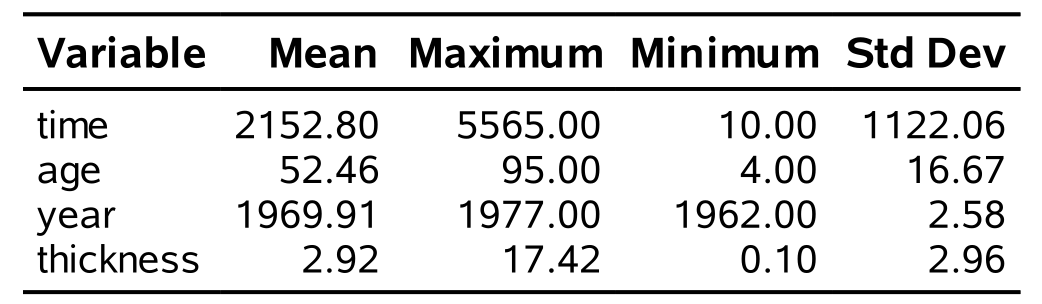
\includegraphics[width = 0.7\textwidth]{img/c7/slides7e10}
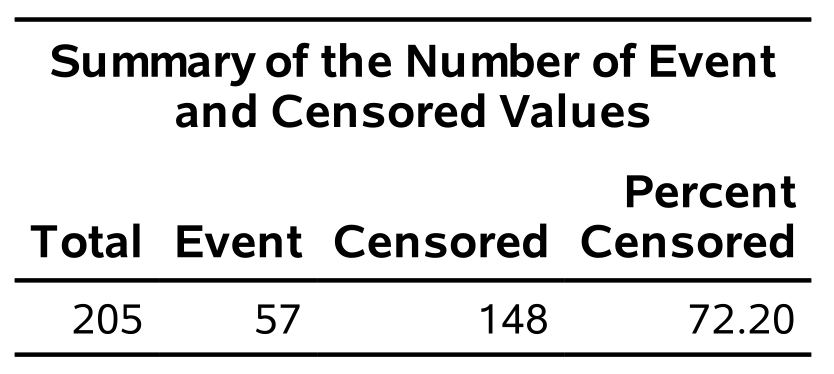
\includegraphics[width = 0.5\textwidth]{img/c7/slides7e11}
\end{center}
\end{frame}

\begin{frame}[fragile]
\frametitle{Cox proportional hazard model for \code{melanoma}}
 The Cox proportional hazards model is 
\begin{align*}
h(t) = h_0(t) \exp( \beta_1 \code{sex} + \beta_2 \code{age} + \beta_3 \code{thickness} + \beta_4 \code{ulcer})
\end{align*}
 We can fit this model in \SASlang{}  using the \code{phreg} procedure:
\vp \vp
\begin{tcolorbox}[colback=white,colframe=hecblue,title=\SASlang{} code for fitting a proportional hazard model]
{\footnotesize 
\begin{verbatim}
proc phreg data=statmod.melanoma;
model time*status(0) = sex age thickness ulcer / ties=exact;
run;
\end{verbatim}
}
\end{tcolorbox}
\end{frame}

\begin{frame}
\frametitle{Likelihood-based tests}
\vp \vp
\begin{center}
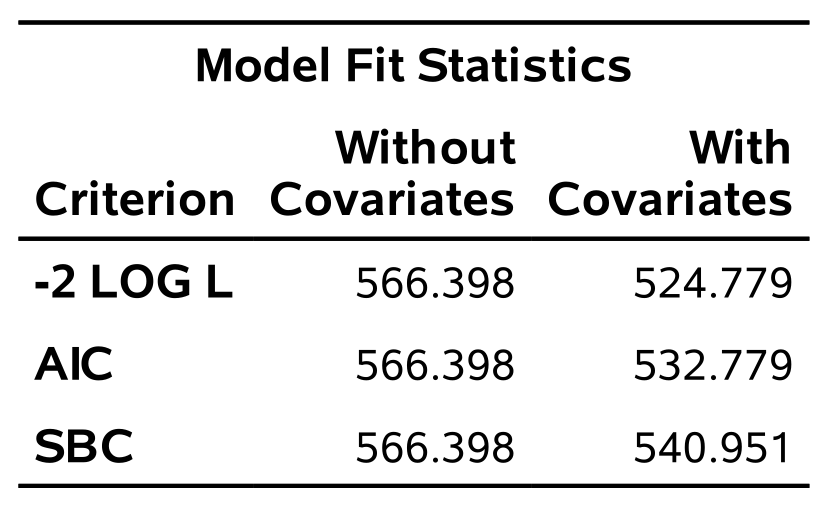
\includegraphics[width = 0.45\textwidth]{img/c7/slides7e12}
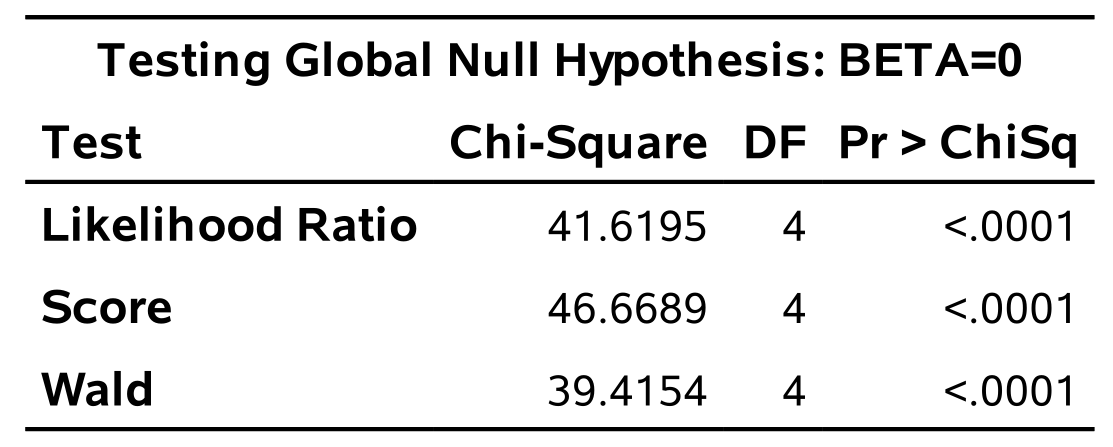
\includegraphics[width = 0.6\textwidth]{img/c7/slides7e13}
\end{center}
{\footnotesize
The output includes the log likelihood value with and without explanatory variables, along with the usual global significance tests for $\Hy_0: \bs{\beta}=\bs{0}_p$ versus $\Hy_a: \bs{\beta} \neq \bs{0}_p$.

}
\end{frame}

\begin{frame}
\frametitle{Estimated coefficients of the Cox model}
\vp \vp
\begin{center}
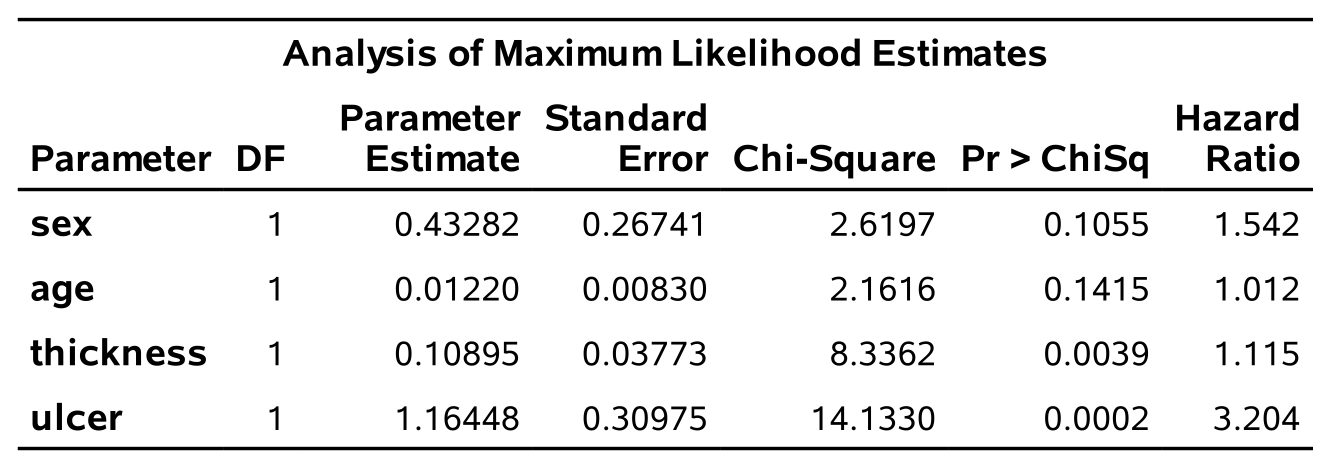
\includegraphics[width = 0.9\textwidth]{img/c7/slides7e14}
\end{center}
% 

\end{frame}

\begin{frame}
\frametitle{Interpretation}
\begin{itemize}
\item For \code{sex}, $\exp(\widehat{\beta}_1)=1.542$ represents the hazard ratio between a man versus a woman of the same age, with the same thickness of tumour and the same ulceration status. Thus, the hazard rate for males is $1.542$ times that for females, \textit{ceteris paribus}.
\item For the variable  \code{thickness}, $\exp(\widehat{\beta}_3)=1.115$. For every $1$mm increase in the tumour thickness, the hazard rate increases by a factor of $1.115$ (or $11.5$\%), when all other variable are held constant. 
\end{itemize}
\end{frame}
% 
% 
% \begin{frame}
% \frametitle{Exemple}
% \textbf{Sortie SAS:}
% \vp \vp
% \begin{center}
% \includegraphics[scale=0.7]{img/c7/mel_cph_2.png}
% \end{center}
% \begin{itemize}
% \item On voit qu'il y a de différents tests pour
% \begin{itemize}
% \vp \vp
% \item[] $\Hy_0: \beta_1 = \cdots = \beta_4 = 0 $
% \item[] $\Hy_1$ au moins un $\beta_j$ est différent de zéro.
% \end{itemize}
% \end{itemize}
% \end{frame}
% 
% \begin{frame}
% \frametitle{Quelques remarques\ldots}
% \begin{align*}
% h_i(t) = h_0(t) \exp(\beta_1 \mathrm{X}_{i1} + \cdots + \beta_p \mathrm{X}_{ip})
% \end{align*}
% \begin{itemize}
% \item Dans le modèle de Cox à risques proportionnels, l'hypothèse sous-jacente est que les effets des variables explicatives sont \alert{constants à travers le temps}. C'est la condition de \alert{risques proportionnels}.
% \begin{itemize}
% \vp \vp
% \item On suppose que l'effet de la variable $\mathrm{X}_j$ sur la fonction de risque $h(t)$ est toujours $\exp(\beta_j)$, peut importe le temps $t$. 
% \item Il y a certainement des situations dans lesquelles cette condition ne sera pas valide. Ex: pour des ages $<18$, les hommes on un taux de risque moins élevé que les femmes, mais pour les ages $\geq 18$, le taux de risque pour les hommes est plus élevés que ceux des femmes.
% \item On peut tester formellement si cette condition est satisfaite, mais on ne verra pas cela.
% \end{itemize}
% \end{itemize}
% \end{frame}

% \begin{frame}
% \frametitle{Quelques remarques\ldots}
% \begin{align*}
% h_i(t) = h_0(t) \exp(\beta_1 \mathrm{X}_{i1} + \cdots + \beta_p \mathrm{X}_{ip})
% \end{align*}
% \begin{itemize}
% \item Dans le modèle de Cox à risques proportionnels, on ne modélise pas la fonction de risque de base $h_0(t)$. 
% \item Rappel: il y a une relation entre la fonction de survie et le taux de risque:
% \begin{align*}
% S(t) = \exp \left\{-\int_0^t h(u) du \right\}
% \end{align*}
% \item Dans le cadre du modèle de Cox à risques proportionnels, on obtient
% \begin{align*}
% S(t) = \exp \left\{-\exp(\beta_1 \mathrm{X}_1 + \cdots + \beta_p \mathrm{X}_p) \int_0^t h_0(u) du \right\}
% \end{align*}
% \item Alors, si on veut estimer la fonction de survie en terme des variables explicatives $\mathrm{X}_1, \ldots, \mathrm{X}_p$, il faudra modéliser la fonction de risque de base $h_0(t)$. 
% \begin{itemize}
% \vp \vp
% \item Il y a plusieurs façons de modéliser $h_0(t)$. On peut le faire de façon non-paramétrique (ex: l'estimateur Kaplan--Meier)\ldots 
% \end{itemize}
% \end{itemize}
% \end{frame}
% 
% \begin{frame}
% \frametitle{Quelques remarques\ldots}
% \begin{itemize}
% \item Il y a plusieurs différents modèles, autres que le modèle de Cox à risques proportionnels, qu'on peut utiliser dans le cadre d'analyse de survie. 
% \item L'analyse de survie est particulièrement difficile, et la présence de la censure rend l'estimation encore plus difficile. 
% \end{itemize}
% \end{frame}




\end{document}
